\section{Results and Discussion}

% From the outline: every result is a table (2 repeats, named baseline) or a figure, then one
% paragraph of discussion. No run ids in the text; they are in the LaTeX comments and in
% configs/thesis_figures.yaml / docs/figures/PROVENANCE.md in the code repository.

% sim_results.tex -- draft of the simulation results (4 Oct 2026).
% Tables are generated by multi_drone_control/tools/thesis_sim_tables.py into Source/src/tables/,
% figures by tools/thesis_sim_figures.py (Images/*.pdf). Run ids: configs/thesis_figures.yaml.
% Cells give the mean over repeats with the number of runs in brackets.

\subsection{Carrying the payload in simulation}
\label{sec:sim_results}

The simulator is the Gazebo rig twin (Section~\ref{sec:simulation}), which reproduces the lab
set-up. It has a 0.86\,kg ring with its magnets at a radius of 0.225\,m, and 0.55\,kg UAVs on
0.55\,m rods of 0.075\,kg that pivot 4\,cm below each airframe. Thrust follows the rig's identified
affine map with battery sag, and the flight controller is a rate loop. Every flight starts
with the ring on the floor. The UAVs take off, swing their rods up to 45$^\circ$, pretension them
and lift the ring to 1.0\,m. Cases are flown twice; the tables give the number of runs in
brackets, so (1) marks a single run.

The height error is $e_z = z_L - z_L^{\mathrm{ref}}$, positive with the ring high, averaged over the
hover. The horizontal error $\|\mathbf{e}_{xy}\|$ is averaged over the first lap of a trajectory. For a
push, the displacement is measured along the push, relative to the mean over the 5\,s before it.

\subsubsection{Tracker initial condition}

Figure~\ref{fig:tracker_x0} and Table~\ref{tab:x0} compare the tracker's relaxed initial condition
($\epsilon = 0.025$) with node~0 pinned to the measurement ($\epsilon = 0$), both without integral
action.

\begin{figure}[h]
\centering
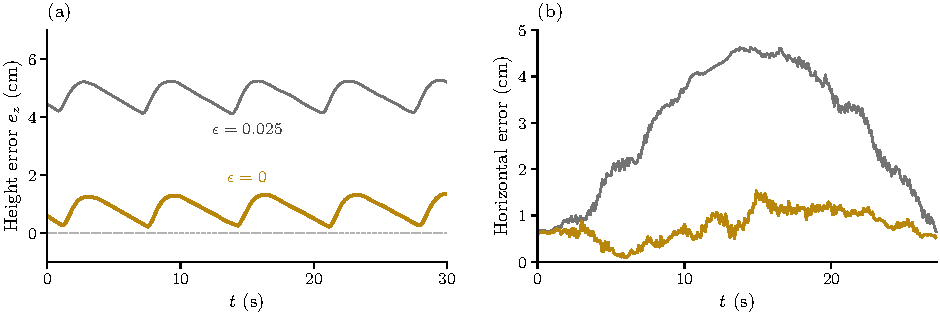
\includegraphics[width=\textwidth]{Images/tracker_x0.pdf}
\caption[Effect of the tracker's initial condition]{Effect of the tracker's initial condition without integral action: node~0 pinned to the
measured state ($\epsilon = 0$, gold) against the relaxed box ($\epsilon = 0.025$, grey). Gazebo rig
twin from a floor start, three UAVs. (a) Hover at 1.0\,m: ring height error from 10\,s after the
lift. Both settings show the same 1\,cm, 7\,s heave. (b) Circle of radius 0.5\,m at 0.125\,m/s:
horizontal ring error over the first lap including its 4\,s spin-up, sampled when the planner's
reference updates (10\,Hz). Dashed in (a): zero error. One run of each case is shown;
Table~\ref{tab:x0} gives the means.}
\label{fig:tracker_x0}
\end{figure}

\begin{table}[h]
\centering
\caption{Ring error with the relaxed and the pinned initial condition, no integral action. The
circle with $\epsilon = 0.025$ is a single run on an earlier code version; its horizontal error
reproduces on the current code (2.8\,cm, with the height integral on).}
\label{tab:x0}
% generated by tools/thesis_sim_tables.py
\begin{tabular}{llcc}
\toprule
Case & Metric & $\epsilon = 0.025$ & $\epsilon = 0$ \\
\midrule
Gazebo, hover at 1.0\,m & height error (cm) & +4.8 (2) & +0.9 (2) \\
Gazebo, circle & horizontal error, mean (cm) & 2.8 (1) & 0.8 (2) \\
 & height error (cm) & +4.8 (1) & +0.8 (2) \\
\bottomrule
\end{tabular}

\end{table}

With the box, each tracker could start its prediction from any state within 2.5\,\% of the
measured one. The solver used that freedom to treat its UAV as closer to the reference than it
was, so small errors were not corrected. Pinning node~0 brings the offset to under 1\,cm. The
remainder is attributed to
the rods' 0.075\,kg mass, which the planner does not model: they hold 52$^\circ$ instead of the
planned 45$^\circ$. This is not yet tested with node~0 pinned. With the box in place, adding the
rods' mass to the planner's model corrected the rod elevation but did not move the height.

\redo{the relaxed box against node~0 pinned on a plant that matches the controller's model (the software-in-the-loop bench, once it flies the twin), three UAVs, hover: whether the box is the whole of the height offset, and whether the rods then hold the planned 45$^\circ$ and tension.}
% --- original text, flown before the rig twin; kept to refill this place:
% With the box, each tracker could start its prediction from any state within 2.5\,\% of the
% measured one. The solver used that freedom to treat its UAV as closer to the reference than it
% was, so small errors were not corrected. In SIL, where the plant matches the model, this was the
% whole of the payload's height offset. Pinning node~0 removes it, and the rods hold the planned
% 45$^\circ$ and the planned tension. In Gazebo the offset drops to under 1\,cm. The remainder is attributed to

The box was a fraction of each \emph{absolute} coordinate, so it widened as the UAVs moved away from
the world origin. The circle's error with the box grows with the ring's distance from the origin,
which is consistent with this (Figure~\ref{fig:tracker_x0}b), although on this circle the distance and
the phase of the lap change together. Pinning node~0 also removes most of that error.

Landing is not yet resolved, with or without the box. In 21 Gazebo flights with $\epsilon = 0$, one
UAV tipped over during landing after the payload had touched down, as 2 of 32 earlier landings with the
box had. Both come from landing, not from the box, and the landing of Section~\ref{sec:sim_landing}
removes them.

\subsubsection{Disturbance rejection}

A constant force was applied to the ring for 15\,s in hover: 0.6\,N downward, about the weight of a
60\,g object, and 0.4\,N horizontally. Both were sized so that the integral stays inside its
bound, at 56\,\% and 51\,\% of it. Without an integral the ring settles 8.4\,cm and 7.6\,cm away, which gives the closed loop's
stiffness to a force on the ring: $K_z = 7.1$\,N/m and $K_{xy} = 5.3$\,N/m, the values used for
$K$ in \eqref{eq:lumped_int}. Figure~\ref{fig:disturbance} shows the model integral on the horizontal push, and
Table~\ref{tab:disturbance} gives both pushes and compares it with the target-shift form.

\begin{figure}[h]
\centering
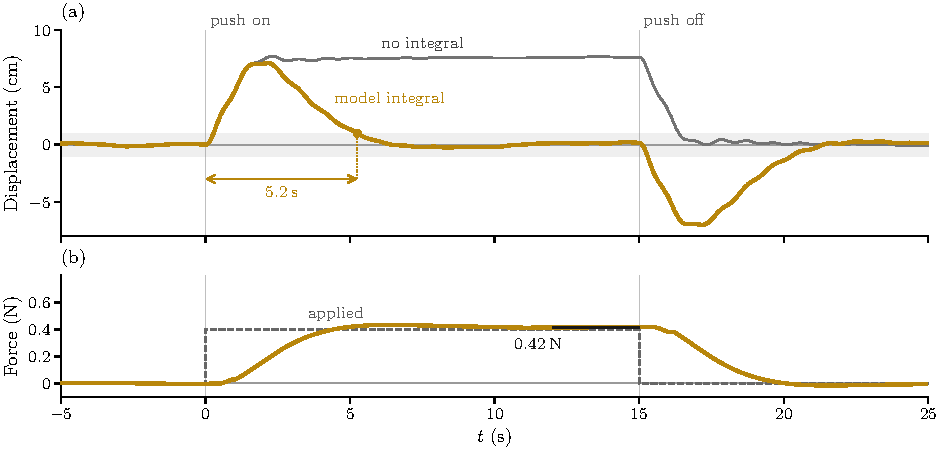
\includegraphics[width=\textwidth]{Images/disturbance.pdf}
\caption[Rejection of a constant force on the ring]{Rejection of a constant force on the ring, Gazebo rig twin, three UAVs, hover at 1.0\,m.
A 0.4\,N horizontal push acts from 0 to 15\,s. (a) Ring displacement along the push, relative to its
mean over the 5\,s before: no integral (grey) and the integral in the planner's model (gold). Band:
$\pm 1$\,cm. Arrow: time for the model integral to bring the ring back within 1\,cm for good. (b)
Change of the model integral's force $\mathbf{d}$ along the push from its value before the push
(gold), against the applied force (dashed). Black bar: its mean over the last 3\,s of the push. The
force holds still for about 0.7\,s after each step, while the ring moves faster than the integral's
5\,cm/s gate. One run of each case is shown; Table~\ref{tab:disturbance} gives the means and the
0.6\,N vertical push.}
\label{fig:disturbance}
\end{figure}

\begin{table}[h]
\centering
\caption{Disturbance rejection in the Gazebo rig twin with $\epsilon = 0$. One of the two
target-shift runs aborted on landing, after the push and its recovery; its push is included. The
change of the integral force is measured from its value before the push (0.06\,N vertically,
0.03\,N horizontally).}
\label{tab:disturbance}
% generated by tools/thesis_sim_tables.py
\small
\begin{tabular}{lccc}
\toprule
 & No integral & Target shift & Model integral \\
\midrule
\multicolumn{4}{l}{\emph{0.6\,N downward push on the ring}} \\
\quad steady displacement (cm) & 8.4 (2) & 0.3 (2) & 0.2 (2) \\
\quad peak displacement (cm) & 8.9 (2) & 6.6 (2) & 6.5 (2) \\
\quad overshoot on release (cm) & 0.4 (2) & 7.1 (2) & 7.0 (2) \\
\quad time to within 1\,cm after onset (s) & -- & 6.0 (2) & 6.1 (2) \\
\quad change of the integral force (N) & -- & -- & 0.58 (2) \\
\midrule
\multicolumn{4}{l}{\emph{0.4\,N horizontal push on the ring}} \\
\quad steady displacement (cm) & 7.6 (2) & n/a & 0.1 (2) \\
\quad peak displacement (cm) & 7.7 (2) & n/a & 7.2 (2) \\
\quad overshoot on release (cm) & 0.1 (2) & n/a & 7.0 (2) \\
\quad time to within 1\,cm after onset (s) & -- & n/a & 5.5 (2) \\
\quad change of the integral force (N) & -- & n/a & 0.42 (2) \\
\midrule
\multicolumn{4}{l}{\emph{One UAV producing more thrust than its map assumes}} \\
\quad height error (cm) & -- & 0.0 (2) & 0.0 (2) \\
\quad horizontal error (cm) & -- & 3.5 (2) & 0.0 (2) \\
\quad ring tilt (\si{\degree}) & -- & 6.4 (2) & 7.9 (2) \\
\bottomrule
\end{tabular}

\end{table}

Both forms of the integral bring the ring back to the target, and on the vertical push their
transients are the same to within a few per cent. With the conversion $K$ set to the measured
stiffness, the loop has the same gain whether the integral moves the target or enters the model. The
force the model integral learns is the force that was applied, within 3\,\% vertically and
4--5\,\% horizontally. Only the model form
acts horizontally, and it removes the horizontal push in the same way.

The integral reduces the peak only partly, by about a quarter vertically (8.9 to 6.5\,cm) and by
7\,\% horizontally (7.7 to 7.2\,cm), because it is slower than the cascade. The ring reaches most
of its uncompensated displacement within about 1\,s, while the integral's time constant is
$1/k_i = 2.5$\,s. When the push ends, the integral still holds the force it learned and drives the
ring past the target by about as much as the push displaced it at onset. This overshoot on release
is a property of integral action, not of where the integral acts. Table~\ref{tab:gain} shows the
trade-off. Doubling $k_i$ reduces the peak by 14\,\%, but the response rings and settles 55\,\% later,
the trend the damping relation of Section~\ref{sec:disturbance} predicts. This is a single run, and its
settling time is sensitive to the 1\,cm threshold against the 1\,cm heave of the hover. Keeping the
ring-speed gate only for the first 5\,s after the lift removes 7--8\,\% with no cost on this push; it has
not yet been flown on a trajectory, a hand-over or a landing.

\begin{table}[h]
\centering
\caption{Integral gain and gate on the 0.6\,N vertical push, model integral. Peak: largest
displacement during the push; overshoot and settling (to within 1\,cm): after it ends. Brackets:
number of runs.}
\label{tab:gain}
% generated by tools/thesis_sim_tables.py
\begin{tabularx}{\textwidth}{Xccc}
\toprule
Model integral & Peak (cm) & Overshoot (cm) & Settling (s) \\
\midrule
$k_i = 0.4$ & 6.5 (2) & 7.0 (2) & 4.7 (2) \\
$k_i = 0.8$ & 5.6 (1) & 6.0 (1) & 7.2 (1) \\
$k_i = 0.4$, speed gate only in the first 5\,s after the lift & 6.0 (1) & 6.4 (1) & 4.5 (1) \\
\bottomrule
\end{tabularx}

\end{table}

When one UAV produces more thrust than its map assumes, both forms hold the height. Only the model
form also removes the horizontal error, and the ring tilts 1.5$^\circ$ further. The thrust error is a
moment on the ring that neither form controls.

\redo{the two forms of the integral with the feedforward to the trackers scaled to 0.9, on a plant that matches the controller's model (the software-in-the-loop bench, once it flies the twin): the planned ring position half a second ahead against the actual one, the rod elevation, and how much of its bound the model integral uses.}
% --- original text, flown before the rig twin; kept to refill this place:
% In SIL the two forms can be compared directly, with the feedforward to the trackers scaled to 0.9.
% Both hold the target, but the reference-shift form raises the height target by 10\,cm and plans a
% climb towards it that never comes: the planned ring position half a second ahead is 4.2\,cm above
% where the ring is. The rods also settle at 48$^\circ$ rather than the planned 45$^\circ$. With the
% model integral the plan predicts what happens (0.0\,cm) and the rods hold 45$^\circ$. In SIL the model
% integral used 89\,\% of its vertical bound (0.95 of 1.07\,N) and raised its warning, because the
% conversion $K$ measured in Gazebo is lower than the SIL plant's stiffness.
% % TODO: generate the SIL plan-prediction numbers from the planner logs as the tables are.

\subsubsection{Other approaches to model error}
\label{sec:sim_methods}
% Sources: docs/overnight_2026-10-04.md (report table), registry R0841-R0955; notes 2026-10-03_*,
% 2026-10-04_* (offset_free_mpc = A, offset_free_innovation, indi_fext, kt_trim, pin_cable_rates,
% ancillary_tracker, l1_ring, xy_stiffness_b3); B4 notes 2026-10-01_load_ext_force (offline replay).
% All flown with the tracker box at 0.025 (before the x0 finding): the +4.8 cm hold is the box.

Before the initial-condition fix, several approaches from the literature were tried against the
steady errors, and each was tested in the same three-UAV rig twin. Three
cases represent the internal errors: the hover itself, and one UAV whose thrust map is wrong in
each direction (its real offset 0.03 above or below the 0.185 its tracker assumes). Two represent
external forces: a 1\,N horizontal push on the ring, and a 0.4\,m/s wind during the orbit.
Table~\ref{tab:methods} gives the results. All of them were flown with the tracker's relaxed initial
condition, so the hover without any correction sits 4.8\,cm high; the comparisons between rows still
hold.

\begin{table}[h]
\centering
\footnotesize
\setlength{\tabcolsep}{4pt}
\caption{Approaches to model error in the Gazebo rig twin (three UAVs, 1.0\,m, floor start; flown
with $\epsilon = 0.025$). Height and horizontal errors in cm, tilt in degrees; one run per cell
unless noted; a dash: not flown. $^{a}$ A UAV tipped during the landing, after the hover, and the fleet
disarmed. $^{b}$ Two runs, agreeing within 0.1.}
\label{tab:methods}
\begin{tabular}{lccccc}
\toprule
 & Hover & One UAV weaker & One UAV stronger & 1\,N push & Wind \\
 & $e_z$ & $e_z$ / $e_{xy}$ / tilt & $e_z$ / $e_{xy}$ / tilt & $e_{xy}$ & $e_{xy}$ \\
\midrule
None & +4.8 & $-$3.0 / 3.8 / 6.7 & +12.8 / 3.5 / 6.0 & 18.0 & 17.9 \\
Height integral (target) & +0.1 & 0.0 / 3.8 / 6.7 & 0.0 / 3.5 / 6.0 & 17.9 & 18.0 \\
Force balance & +3.8 & +3.9 / 1.3 / 9.0 & -- & 0.3 & 3.9 \\
Force balance + height int. & +0.1$^{b}$ & 0.0 / 1.3 / 9.0$^{b}$ & -- & 0.4$^{b}$ & 3.9$^{b}$ \\
Offset-free observer & +1.6 & +1.0 / 0.2 / 8.0 & +2.4 / 0.1 / 7.5 & 2.6$^{b}$ & 7.8$^{b}$ \\
Measured cable force & +4.2$^{a}$ & +3.8 / 3.1 / 0.8$^{a}$ & +4.5 / 0.6 / 0.3 & -- & -- \\
Measured force + height int. & 0.0$^{a}$ & 0.0 / 3.1 / 0.8 & 0.0 / 0.6 / 0.3$^{a}$ & -- & -- \\
Thrust-gain trim & +3.7 & +4.1 / 1.3 / 2.3 & -- & -- & -- \\
Rod mass in the planner & +5.0 & -- & -- & -- & -- \\
\bottomrule
\end{tabular}
\end{table}

\begin{description}
    \item[Height integral on the target.] Zeroes the height in every case and does nothing
    horizontally: the push and the wind still move the ring 18\,cm.
    \item[Force balance.] Estimates a constant force on the ring and one shared by the UAVs from
    the measured motion and the delivered thrust, and gives them to the planner's model
    \cite{muske2002disturbance}. It removes the push and most of the wind. It cannot see the internal
    height offset: by Newton's law, a force that the system exerts on itself does not appear in its
    total. It books a UAV's thrust-map error as a force on the ring, and leans the formation into
    it, which tilts the ring further. Combined with the height integral it was the best on height and
    external forces. Its transients were not small: on the push it peaked at 14.5\,cm, and on release
    it overshot by 14.8\,cm and tilted the ring 7.1$^\circ$.
    \item[Offset-free observer.] Estimates the force from the planner's own prediction error, as in
    offset-free MPC \cite{pannocchia2003disturbance}. It helped everywhere but converged slowly and left
    residuals, because a small offset shows up in the plan's cable states rather than in the payload's
    predicted motion.
    \item[Measured cable force.] Each tracker takes the cable force from its measured acceleration
    and delivered thrust, the ground-side counterpart of the IMU-based compensation of
    \cite{tudelft}. It was the only approach that levelled the ring against one UAV's wrong thrust
    map (0.3--0.8$^\circ$ against 6--7$^\circ$), because it corrects each UAV's own force. In four of
    six runs, however, a UAV tipped during the landing.
    \item[Thrust-gain trim.] A per-UAV estimate of the throttle-to-acceleration gain, from the UAV's
    own measured acceleration and its static share of the cable force. It partly corrects a wrong map.
    \item[Rod mass in the planner.] Corrected the rods' elevation (49.7 to 42.8$^\circ$ against a planned
    45$^\circ$) but not the height.
\end{description}
Further candidates were rejected before flying, because tests on logged flights showed they would
not work. These were pinning the cable rates at node~0, a thrust reference weight in the
tracker, and an $\mathcal{L}_1$ adaptive force estimate \cite{hovakimyan2010l1} at the planner's
10\,Hz rate. Raising the planner's weight on the ring's horizontal position by three and by ten times
cut the push displacement only by 23 and 38\,\% (18.5 to 14.3 and 11.4\,cm), and the higher weight
rocked the ring by 6$^\circ$. Aiming the rods at the hand-over angle instead of 45$^\circ$ made it
worse (20.7\,cm). Both were removed.

Two conclusions carried forward. First, the internal height offset was not a force at all, which is
why no force estimate could find it; it turned out to be the tracker's initial condition.
Second, a wrong thrust map on one UAV is a moment on the ring, and only a correction of that UAV's own
force removes the tilt it causes. A force on the ring, estimated or integrated, can only move the
whole formation.

\subsubsection{Trajectories}

Table~\ref{tab:traj} gives the tracking of each reference kind of Section~\ref{sec:trajectories} in
the rig twin with $\epsilon = 0$, three or four UAVs from a floor start. The integral action was off,
so the height column is the static offset that the height integral removes
(Section~\ref{sec:disturbance}). The horizontal error stays about a centimetre on average and under
3\,cm at worst for every reference, with three UAVs or four. The spin turns the ring once about its
vertical axis while it circles, and the ring follows that yaw within a few degrees.

\begin{table}[htbp]
\centering
\caption[Trajectory tracking]{Trajectory tracking in the Gazebo rig twin, $\epsilon = 0$, no integral
action, ring at 1.0\,m, floor start. Four UAVs fly the even ring except in the four-UAV hover, which
uses the detach layout. Speed: the commanded speed, which the line and the spin reach at their
peak. Horizontal error per sample, sampled where the planner's reference updates, over the motion
(the circle's first lap) or the 15\,s before LAND (hover); height error and tilt: means over the
same window; each cell is the mean over the runs.}
\label{tab:traj}
% generated by tools/thesis_sim_tables.py
\begin{tabularx}{\textwidth}{>{\raggedright\arraybackslash}Xccccccc}
\toprule
 & & Speed & \multicolumn{2}{c}{Horizontal error (cm)} & Height & Tilt & \\
\cmidrule(lr){4-5}
Reference & UAVs & (m/s) & mean & max & error (cm) & (\si{\degree}) & Runs \\
\midrule
Hover & 3 & -- & 0.7 & 0.7 & $+$0.9 & 1.2 & 2 \\
Hover, plates 1/3/5/9 & 4 & -- & 0.6 & 0.7 & $-$2.2 & 1.6 & 2 \\
Line, 1\,m shuttle & 4 & 0.25 & 0.9 & 2.7 & $-$1.7 & 1.3 & 2 \\
Circle, $r = 0.5$\,m & 3 & 0.125 & 0.8 & 1.5 & $+$0.8 & 1.2 & 6 \\
Circle, $r = 0.5$\,m & 4 & 0.125 & 0.9 & 1.9 & $-$1.7 & 1.3 & 2 \\
Figure-8, 2\,m $\times$ 1\,m & 4 & 0.25 & 0.8 & 2.4 & $-$1.7 & 1.3 & 2 \\
Spin, circle with one turn of yaw$^a$ & 4 & 0.125 & 0.5 & 1.4 & $-$1.7 & 1.2 & 2 \\
\bottomrule
\multicolumn{8}{l}{\footnotesize $^a$ Yaw error 1.3\,\si{\degree} mean, 3.5\,\si{\degree} max over the turn.}
\end{tabularx}

\end{table}

The circle and the figure-8 were also flown with the relaxed box of
Section~\ref{sec:sim_results}, $\epsilon = 0.025$ (Figure~\ref{fig:traj}). Pinning node~0 cut the
horizontal error over the motion from 3.0 to 1.0\,cm on the circle and from 2.9 to 0.8\,cm on the
figure-8, and the height error from $+3.2$ to $-1.7$\,cm. The relaxed box's error grows as the ring
moves away from the world origin and shrinks as it returns, in both shapes.

\begin{figure}[h]
\centering
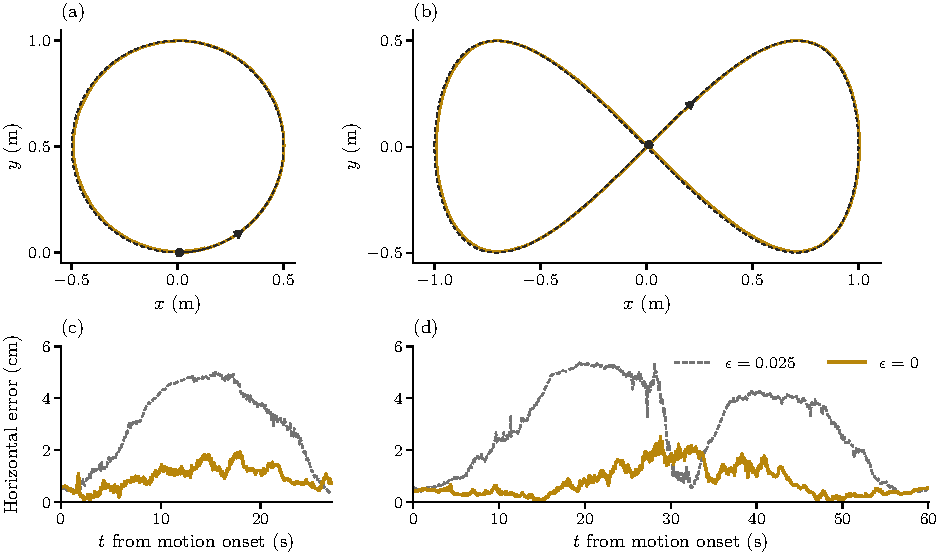
\includegraphics[width=\textwidth]{Images/trajectories.pdf}
\caption[Trajectory tracking with four UAVs]{Pinning node~0 cuts the four-UAV trajectory error by about
a factor of three. (a) Circle of radius 0.5\,m, one lap of 27\,s including a 4\,s spin-up; (b) a
2\,m\,$\times$\,1\,m figure-8 in 60\,s. Gold: ring path with $\epsilon = 0$; dark dashed: reference;
dot and arrow: start and direction. (c, d) Horizontal ring error from the onset of motion, sampled
when the planner's 10\,Hz reference updates, with $\epsilon = 0$ (gold) and the relaxed box
($\epsilon = 0.025$, dashed). Gazebo rig twin, four UAVs on the even ring, ring at 1.0\,m; one run of
each.}
\label{fig:traj}
\end{figure}

\subsubsection{Landing}
\label{sec:sim_landing}

Figure~\ref{fig:landing} compares a straight descent with the landing of
Section~\ref{sec:takeoff}, and Table~\ref{tab:land} gives every landing flown in the rig twin
with $\epsilon = 0$: three and four UAVs, hover, the pushes, the thrust-map errors, the circle and the
detach. With a straight descent, 2 of 21 landings tipped a UAV past 45$^\circ$. With the unwind alone
the outward push was gone but 2 of 18 still tipped: one survivor oscillated when the cable term
stepped off, and one departed UAV rocked on the floor. With the feedforward ramp and the ground idle
added, none of 18 tipped.

\begin{figure}[h]
\centering
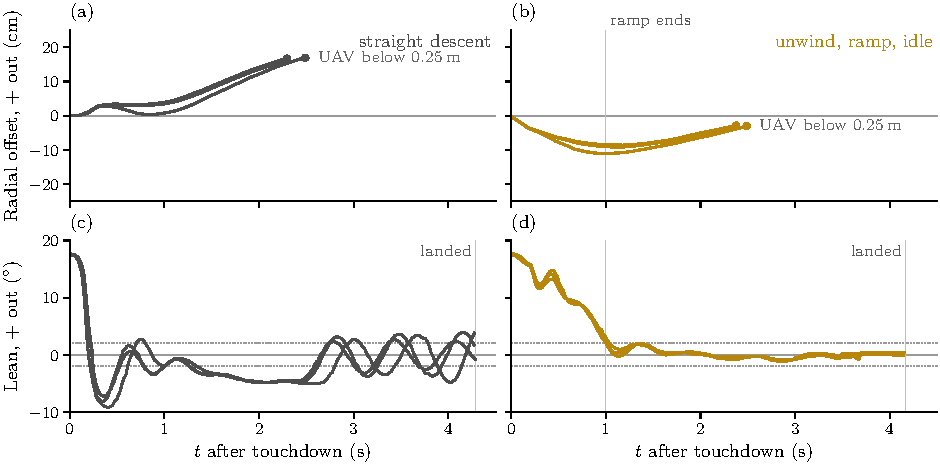
\includegraphics[width=\textwidth]{Images/landing.pdf}
\caption[Landing after touchdown]{Landing after the payload touches down, Gazebo rig twin, three
UAVs (interchangeable; one run of each). (a, c) Straight descent, with the cable feedforward cut at
touchdown. (b, d) Unwind along the rods, a 1\,s feedforward ramp and idle on the floor. (a, b) Radial
offset of each UAV from its reference about the ring centre, positive outward, drawn until the UAV
is below 0.25\,m (dot), below which its reference follows it. (c, d) Lean of each UAV's thrust axis
along its outward radial; the 17.5$^\circ$ at touchdown is the lean against the rod's pull. Dotted:
$\pm 2^\circ$. In a straight descent the rods push the UAVs outward, still growing at 17\,cm, and the
UAVs keep rocking until they land. With the unwind they trail their outward-moving reference instead
and settle within $\pm 2.6^\circ$ once the ramp ends.}
\label{fig:landing}
\end{figure}

\begin{table}[h]
\centering
\caption{Every landing in the Gazebo rig twin with $\epsilon = 0$, from load-down until the fleet is
declared landed. Tipped: a UAV past 45$^\circ$; the fleet aborts at 60$^\circ$. The ranges are over
the landings without a tip.}
\label{tab:land}
% generated by tools/thesis_sim_tables.py
\begin{tabularx}{\textwidth}{>{\raggedright\arraybackslash}Xcccc}
\toprule
Landing & Runs & Tipped (aborted) & Pushed outward (cm) & Tilt after 1.2\,s (\si{\degree}) \\
\midrule
straight descent & 21 & 2 (1) & 5.4--18.2 & 2.2--5.7 \\
unwind & 18 & 2 (2) & 0.5--4.1 & 2.4--5.0 \\
unwind, feedforward ramp, ground idle & 18 & 0 (0) & 0.5--3.0 & 1.8--4.0 \\
\bottomrule
\end{tabularx}

\end{table}



% sim_detach.tex -- Results: detach in simulation (draft 4 Oct 2026). No run ids in the text.
% Runs: OCP vs network R0111-R0114 (6 Aug, 0.4 kg payload, 0.5 m cables, circle 0.6 m/s);
% hand-back R0093 (even ring, 62 deg), R0108/R0109; SIL mode study R0496-R0505 (25 Sep);
% layout R0559-R0572 (hover) and R0554/R0556 (mid-circle) (25 Sep, legacy
% linear plant, 0.86 kg ring, 0.5 m rods, 0.64 kg UAVs); 1/3/6/9 R0582/R0584; LAND v4 R0571/R0572;
% rig twin W4 rehearsal R0939 (4 Oct, 0.55 m rods, 0.55 kg UAVs, affine map, old tracker box).
% Restructured 9 Oct (structure audit): opens with its question, baseline and bar; order layout,
% transient, against the network, rig; the freed UAV's own landing added (fig:departed_landing) with
% pending rig figures.

\subsection{Detach}
\label{sec:sim_detach}

This section answers the leave half of RQ1: does a detach by OCP resize keep the ring level when one UAV
of four leaves? The baseline is a hand-off of the payload to the dissipative network on the same
detach, and for the geometry the even layout; the bar is the ring's tilt back under the hover's own
maximum plus 0.5$^\circ$ (Table~\ref{tab:detach}).

\paragraph{Layout.}
\redo{detach layout study, four UAVs to three in hover, the UAV on plate~3 released, two runs per layout: the even ring (plates 0/3/6/9) against plates 1/3/5/9 (peak and settled tilt); the 1/3/5/9 detach in the middle of a circle; plates 1/3/6/9 (clearance of the departing UAV against tilt and throttle).}
% --- original text, flown before the rig twin; kept to refill this place:
% \paragraph{Layout.} The geometric condition of Section~\ref{sec:reconfig} was tested directly. Four
% UAVs on an even ring (plates 0/3/6/9) and on plates 1/3/5/9 hovered, and the UAV on plate~3 was
% released. On the even ring the three survivors' attachment points have the ring's centre of mass on
% the edge of their support triangle, and the payload swung to a 25.6--28.5$^\circ$ peak and settled at
% 6.7--6.8$^\circ$. On plates 1/3/5/9 the survivors form an even triangle: the peak was
% 3.0--3.3$^\circ$ and the payload settled at 0.1--0.2$^\circ$ (Table~\ref{tab:detach_layout}). The same
% detach in the middle of a circle peaked at 6.9--7.7$^\circ$ and settled at 0.3$^\circ$, and the
% survivors continued the circle. Moving one more UAV, to plates 1/3/6/9, gives the departing UAV more
% room (0.82\,m to its nearest neighbour instead of 0.58\,m) at a cost of 2.5$^\circ$ of peak tilt,
% 0.45$^\circ$ of settled tilt and 10\,\% more throttle on one survivor.
%
% \begin{table}[h]
% \centering
% \caption{Detach from four UAVs to three in hover, Gazebo, 0.86\,kg ring, by layout. Two runs per layout.}
% \label{tab:detach_layout}
% \begin{tabular}{lcc}
% \toprule
% Layout (plates) & Peak tilt after DETACH & Settled tilt \\
% \midrule
% Even, 0/3/6/9 & 25.6--28.5$^\circ$ & 6.7--6.8$^\circ$ \\
% 1/3/5/9 & 3.0--3.3$^\circ$ & 0.1--0.2$^\circ$ \\
% 1/3/5/9, mid-circle & 6.9--7.7$^\circ$ & 0.3$^\circ$ \\
% \bottomrule
% \end{tabular}
% \end{table}

\paragraph{The transient.} Figure~\ref{fig:detach} shows one detach in the rig twin: four UAVs on plates 1/3/5/9 in hover, the
UAV on plate~3 released, with $\epsilon = 0$. The uneven 1/3/5/9 layout loads the UAV on plate~9 most.
At DETACH the planner, re-solved for the three survivors on their actual plates, hands the released
UAV's load to them in one 0.1\,s tick. The ring tilts by at most 3.3$^\circ$ and is back within its
hover band after 1\,s.

\begin{figure}[h]
\centering
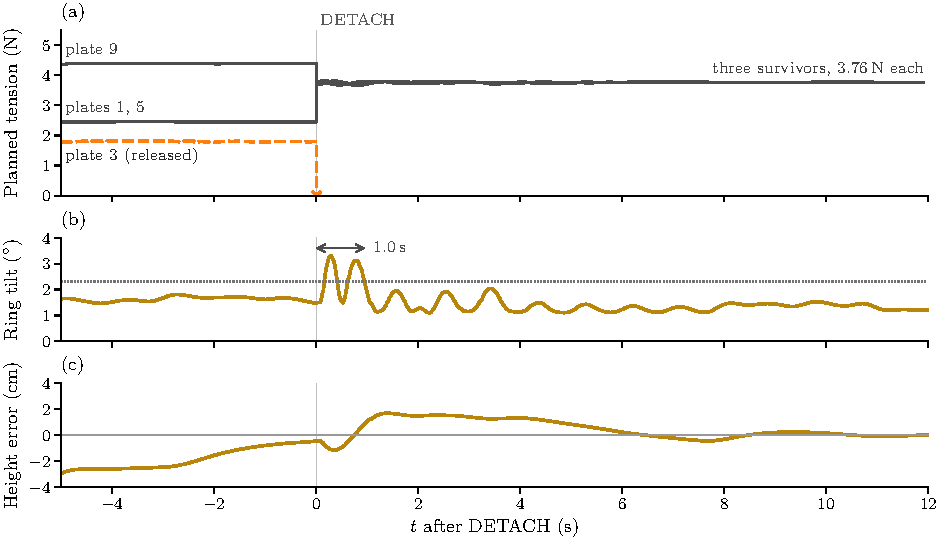
\includegraphics[width=\textwidth]{Images/detach.pdf}
\caption[Detach by OCP resize]{Detach of one UAV of four by OCP resize, Gazebo rig twin, hover at
1.0\,m, UAVs on plates 1, 3, 5 and 9 (Figure~\ref{fig:geometry}). (a) Rod tension planned for each
UAV; the UAV on plate~3 (dashed) is released at DETACH, and the three survivors, now an even
triangle, share the load equally. (b) Ring tilt; dotted: the hover's own maximum plus 0.5$^\circ$;
arrow: time until the tilt stays below it. (c) Ring height error against the 1.0\,m target. One run;
the tensions are planned, since the rig twin does not measure them.}
\label{fig:detach}
\end{figure}

\paragraph{Repeats.} Table~\ref{tab:detach} gives the same detach over five runs with $\epsilon = 0$,
against the earlier rehearsal, which differed in two ways: the relaxed box and the height integral on.
With $\epsilon = 0$ every run peaks at a few degrees and is back within its hover band in about a
second, and the five runs agree closely.

\begin{table}[htbp]
\centering
\caption[Detach, repeats]{Detach of one UAV of four in hover by OCP resize, Gazebo rig twin, plates 1,
3, 5 and 9, ring at 1.0\,m. Peak tilt: in the 5\,s after DETACH. Back in band: time until the tilt
stays under the hover's own maximum plus 0.5$^\circ$. Height change: largest change from the mean
height before DETACH, in the 12\,s after. Ranges over the runs.}
\label{tab:detach}
% generated by tools/thesis_sim_tables.py
\begin{tabularx}{\textwidth}{>{\raggedright\arraybackslash}Xcccc}
\toprule
 & & Peak tilt & Back in band & Height change \\
Tracker box & Runs & (\si{\degree}) & (s) & (cm) \\
\midrule
$\epsilon = 0.025$, height integral on & 1 & 3.2 & 2.6 & 2.7 \\
$\epsilon = 0$, no integral & 5 & 2.8--4.0 & 0.9--1.0 & 3.4--3.6 \\
\bottomrule
\end{tabularx}

\end{table}

\paragraph{OCP resize against network hand-off.}
\redo{OCP resize against network hand-off on the same detach, four UAVs to three during a circle (and in hover): settled payload tilt and the survivors' tracking error; with it the network's hand-back to the planner, with and without the two fixes (no soft-start restart on an airborne hand-back, solver primed before it flies).}
% --- original text, flown before the rig twin; kept to refill this place:
% \paragraph{OCP resize against network hand-off.} Table~\ref{tab:detach_ab} compares the two detach
% methods of Section~\ref{sec:reconfig} on the same flight: four UAVs flying a circle, one released
% mid-way. The flights used an early payload (0.4\,kg, 0.5\,m cables, circle at 0.6\,m/s). With the OCP
% resize the payload settled level and the survivors kept tracking their references. With the network
% hand-off the payload settled tilted by 26--48$^\circ$, and the survivors were 0.06--0.91\,m off their
% references while the network redistributed the load. Two fixes were needed for the network sequence
% to hand back to the planner at all: the feedforward soft-start must not restart on an airborne
% hand-back, and the new solver must be primed before it flies. Without them the payload dropped to
% 0.07\,m above the floor after the detach; with them it stayed above 0.46\,m.
%
% \begin{table}[h]
% \centering
% \caption{Detach from four UAVs to three during a circle, Gazebo, early payload (0.4\,kg).}
% \label{tab:detach_ab}
% \begin{tabular}{lcc}
% \toprule
%  & OCP resize & Network hand-off \\
% \midrule
% settled payload tilt & about 1$^\circ$ & 26--48$^\circ$ \\
% survivor tracking error & about 1\,mm & 60--910\,mm \\
% \bottomrule
% \end{tabular}
% \end{table}

\redo{the same comparison on a plant that matches the controller's model (the software-in-the-loop bench, once it flies the twin), hover and circle: payload tilt after the detach with the network against the OCP resize.}
% --- original text, flown before the rig twin; kept to refill this place:
% On the 0.86\,kg ring the gap widened. In the software-in-the-loop bench the network aborted the
% flight at 53--61$^\circ$ of payload tilt after a detach, both in hover and in the circle, while the
% OCP resize held the survivors level to within 0.5--2$^\circ$.

\paragraph{On the rig.} The detach was flown on the rig on 8 October, in four flights.
Figure~\ref{fig:rig_detach} sets their ring tilt and height error after the release against the twin.

\pendingfig{fig:rig_detach}{Detach on the rig against the twin: ring tilt and height error after the release for the announced, unannounced and 150-degree-gap detaches; rig gold, twin repeats grey.}{built from the 8 Oct rig runs (next)}

\paragraph{The freed UAV's own landing.} After a detach the freed UAV lands by itself, off the ring
(Section~\ref{sec:reconfig}). On the rig on 8 October this landing did not finish: in all four detach
flights the freed UAV floated above its resting height until the fleet's disarm at the end of the
landing dropped it about 0.3\,m (Figure~\ref{fig:departed_landing}a), and the twin shows the same stall
(Figure~\ref{fig:departed_landing}b). Its landing was therefore changed: its height reference is pushed
down to its own resting height, and once it is there it is disarmed alone, without waiting for the
fleet (Figure~\ref{fig:departed_landing}c, in the twin). Figure~\ref{fig:rig_departed} shows the
change on the rig.

\begin{figure}[htbp]
\centering
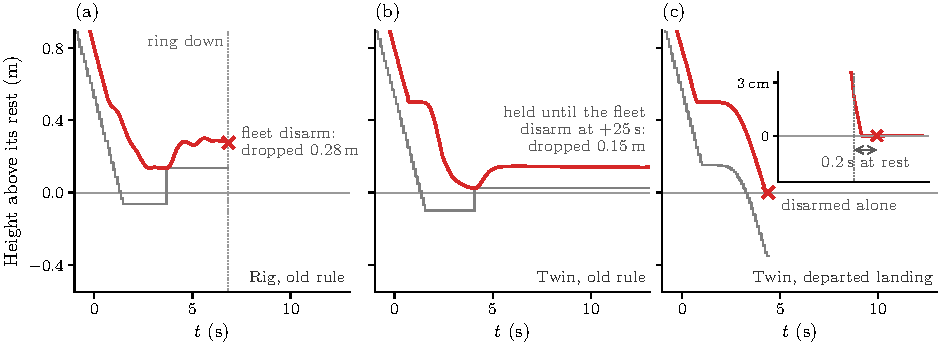
\includegraphics[width=\textwidth]{Images/departed_landing.pdf}
\caption[A freed UAV's own landing, old rule and departed landing]{A UAV landing by itself off the ring, the same UAV (QUAD4) in three cases, aligned where it passes 0.8\,m on the way down; solid: its height above its own resting height, grey: its height reference until it is disarmed, cross: its disarm, dotted: the ring reaching the floor. (a) Rig, old rule: its touchdown test fired 0.14\,m above its rest, the reference froze there, the UAV rose to 0.28\,m and hovered until the fleet's disarm at the end of the landing dropped it 0.28\,m. (b) Twin, old rule: the same stall, held 0.15\,m up for 25\,s until the fleet's disarm dropped it. (c) Twin, departed landing: the reference is pressed below the resting height until the UAV is there, and it is disarmed alone 0.2\,s after reaching it (inset). The plateau at 0.5\,m in (b) and (c) is the UAV standing on the tip of its rod before the rod tips over.}
\label{fig:departed_landing}
\end{figure}

\pendingfig{fig:rig_departed}{The freed UAV's own landing on the rig with the departed landing: pushed to its resting height and disarmed alone.}{rig W4/W5, 14 Oct}

\paragraph{Fewer than three.} Detaching from three UAVs to two is not attempted. A rigid payload on two
rim points is a pendulum about the line between them, and its centre of mass hangs off that line.
The planner refuses a detach that would leave fewer than three
UAVs.

\redo{a detach from three UAVs to two, to show the payload capsizing on two rim points.}
% --- original text, flown before the rig twin; kept to refill this place:
% In the bench the payload capsized. The planner refuses a detach that would leave fewer than three


% sim_attach.tex -- Results: attach in simulation (draft 4 Oct 2026). No run ids in the text.
% Runs: network attach demo R0196/R0197, R0203/R0204, R0209 (storyboard), R0234, R0243 (10 Sep,
% 0.6 kg ring); layouts R0234, R0266-R0272; weld ladder R0126-R0141 (9 Aug); OCP attach SIL
% R0518-R0521, Gazebo R0541-R0552, R0575/R0577, R0580/R0581 (25 Sep); M1 R0646 (baseline),
% R0685/R0686, Wesley watched R0687 (27 Sep); combined M1 R0696/R0697, R0699 canonical;
% M2 T0015-T0029, bench R0707-R0720. Legacy worlds: 0.86 kg ring,
% 0.5 m rods, 0.64 kg UAVs, linear thrust map, tracker box 0.025 (all before 4 Oct).
% FIGURE TODO: rebuild the storyboard on the M1 rejoin (R0685) with tools/attach_storyboard.py.

\subsection{Attach}
\label{sec:sim_attach}

The attach was developed in three stages: a network-based attach, the attach by OCP resize, and the
full rejoin mission with the collaborator's approach controller. None has yet been flown on the rig
twin or the rig.

\subsubsection{Network attach}

\redo{the network attach during a circle at 0.2\,m/s: three UAVs at 3, 12 and 9 o'clock, ATTACH holds the target, a fourth UAV welds at 6 o'clock and is handed out by the dissipative network. With it the storyboard figure (the fleet at four instants, the plan view of the approach, the ring tilt against time).}
% --- original text, flown before the rig twin; kept to refill this place:
% The first attach demonstration (Figure~\ref{fig:attach}) used a 0.6\,kg ring. Three UAVs at 3, 12 and
% 9 o'clock flew a circle at 0.2\,m/s; ATTACH held the target, and a fourth UAV welded at 6 o'clock and
% was handed out by the dissipative network.
%
% \begin{figure}[h]
% \centering
% 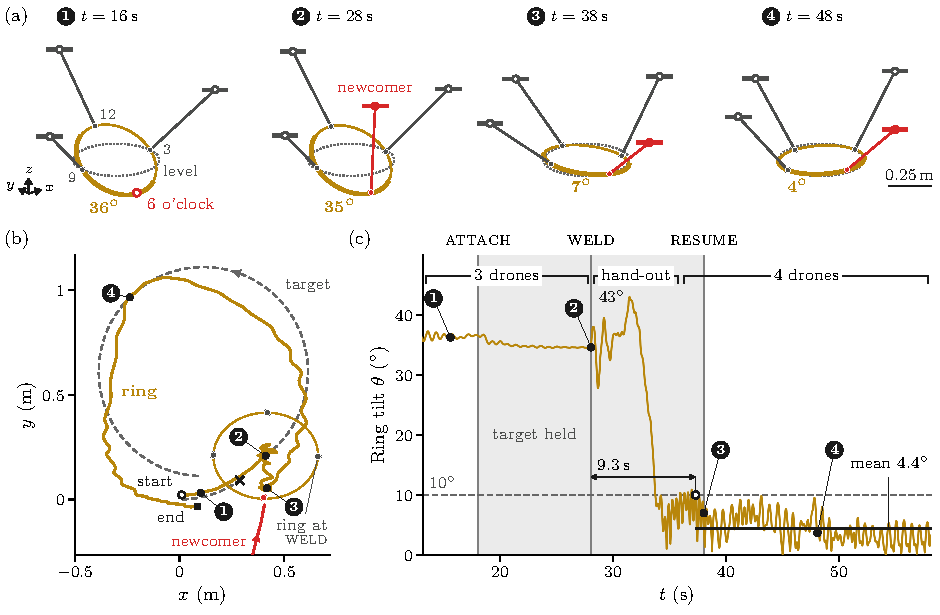
\includegraphics[width=\textwidth]{Images/attach_storyboard.pdf}
% \caption[Attach during a circle]{Attach during a circle in Gazebo (0.6\,kg ring of radius 0.25\,m on 0.5\,m rods). (a) The
% fleet at the four numbered instants, rebuilt from the logged poses in one orthographic view: carriers
% grey, newcomer red; thick: near half of the ring; dotted: the ring if it were level; bar: 0.25\,m.
% (b) Plan view of the ring centre (gold; circle: start, square: end), the payload target (dashed; x:
% held from ATTACH) and the newcomer's approach (red), with the ring and its rim anchors at the weld.
% (c) Ring tilt; grey band: target held; dashed: 10$^\circ$. Three UAVs at 3, 12 and 9 o'clock start
% the circle with the ring tilted by 34--37$^\circ$. ATTACH holds the target and the newcomer welds to
% the empty 6 o'clock rim. During the 8\,s hand-out the tilt first rises to 43$^\circ$; from 9.3\,s
% after the weld it stays under 10$^\circ$ (mean 4.4$^\circ$, peak 9.96$^\circ$), and the four UAVs fly
% the rest of the circle, 0.20\,m RMS from the target against 0.02\,m with three.}
% \label{fig:attach}
% \end{figure}

\redo{the network attach by layout, 3/12/9 o'clock against 4/12/8 o'clock with the newcomer at 6: three-UAV hover tilt, weld transient and four-UAV circle tilt, and the load share of the UAV at 12 o'clock.}
% --- original text, flown before the rig twin; kept to refill this place:
% The sequence completed in every repeat, but it exposed two limits. First, three UAVs on a ring hang it
% tilted when their attachment points leave the centre of mass on the edge of their support triangle:
% at 3/12/9 o'clock the ring hung 27--37$^\circ$ before the weld. The fourth UAV is what levels it.
% Second, the layout trades a level hover against a level circle (Table~\ref{tab:attach_layout}). At
% 3/12/9 o'clock plus 6 the hover is tilted and the four-UAV circle is level. At 4/12/8 o'clock plus 6
% the hover is level, but the UAV at 12 o'clock carries about 40\,\% of the load against 20\,\% for the
% others, and the four-UAV circle rolled by 20--37$^\circ$. A tracker without an integrator sags in
% proportion to its force error, so the most heavily loaded UAV sags most, and a common-mode trim cannot
% correct a differential sag.
%
% \begin{table}[h]
% \centering
% \caption{Network attach on the 0.6\,kg ring by layout (Gazebo).}
% \label{tab:attach_layout}
% \small
% \begin{tabularx}{\textwidth}{>{\raggedright\arraybackslash}Xccc}
% \toprule
% Layout & Three-UAV hover tilt & Weld transient & Four-UAV circle tilt \\
% \midrule
% 3/12/9 o'clock, newcomer at 6 & 33$^\circ$ & 47$^\circ$ peak, 12\,s to settle & 3.7$^\circ$ mean \\
% 4/12/8 o'clock, newcomer at 6 & 2.0$^\circ$ & 10$^\circ$ mean over 4\,s & 20--37$^\circ$ roll \\
% \bottomrule
% \end{tabularx}
% \end{table}

\paragraph{The weld itself.}
\redo{the joint ladder at the weld (ball joint, rod with its inertia, rod with a mid-span joint, rigid weld): flight time after the weld and payload tilt 2\,s and 8\,s after it.}
% --- original text, flown before the rig twin; kept to refill this place:
% \paragraph{The weld itself.} An early hypothesis was that the weld transient came from the
% compliance of the joint between rod and ring. Table~\ref{tab:weld} shows the joint ladder flown to test
% it. A ball joint, a rod with its real inertia and a rod with an extra mid-span joint all behaved alike,
% and a rigid, moment-transmitting weld capsized the payload within 2\,s in five runs out of five.
% Compliance was therefore not the cause. The transient came from the incumbents' tensions stepping to
% their new solution in one tick at the weld, which was then replaced by a blend over the hand-out. The
% attachment is modelled as a ball joint from then on.
%
% \begin{table}[h]
% \centering
% \caption{Payload tilt after the weld by joint model (Gazebo, early attach).}
% \label{tab:weld}
% \small
% \begin{tabularx}{\textwidth}{>{\raggedright\arraybackslash}Xccc}
% \toprule
% Joint at the weld & Flight after the weld (s) & Tilt at +2\,s & Tilt at +8\,s \\
% \midrule
% Ball & 10.1--10.2 & 46--49$^\circ$ & 31--34$^\circ$ \\
% Rod with inertia & 10.4 & 47$^\circ$ & 36$^\circ$ \\
% Rod with mid-span joint & 10.0--10.3 & 40--44$^\circ$ & 26--35$^\circ$ \\
% Rigid & 1.7--1.9 (5 of 5 capsized) & 83--106$^\circ$ & -- \\
% \bottomrule
% \end{tabularx}
% \end{table}

\subsubsection{Attach by OCP resize}

\redo{network attach against attach by OCP resize at the same weld, in hover and in the middle of a circle, on a plant that matches the controller's model (the software-in-the-loop bench, once it flies the twin): payload tilt after the weld.}
% --- original text, flown before the rig twin; kept to refill this place:
% On the 0.86\,kg ring the network attach capsized the payload within about 8\,s of every weld in the
% software-in-the-loop bench, while the OCP resize held the same weld at a peak of about 10$^\circ$, in
% hover and in the middle of a circle. The attach was therefore moved to the OCP resize.

\redo{the attach by OCP resize in Gazebo: the full sequence (approach, weld, resize, resume) in hover; a rejoin during the circle, two runs (weld peak, tilt with four UAVs on the circle, landing); the newcomer's rod pivot below its centre of mass, which the twin has on every UAV; the newcomer's reference aimed along the line to the incumbents' cable apex.}
% --- original text, flown before the rig twin; kept to refill this place:
% In Gazebo the newcomer then flipped 2--5\,s after the weld in every run. The cause was a lever the
% model did not have: the newcomer's arm pivoted 5\,cm below its centre of mass, so the rod's pull,
% modelled at the centre, produced a moment the newcomer's rate loop could not hold. With the pivot at
% the centre, as on the other UAVs, the full sequence (approach, weld, resize, resume) ran clean, with a
% weld peak of 11.6$^\circ$ settling to 0.8$^\circ$. A rejoin during the circle then completed in two
% runs out of two: weld peaks of 10.3--10.5$^\circ$, 0.8--0.9$^\circ$ with four UAVs on the circle, and
% a clean landing. A further correction made the newcomer take its balanced share of the load, aiming
% its reference along the line to the incumbents' cable apex; the weld peaks were then
% 10.7--11.9$^\circ$.

\subsubsection{The rejoin mission}

\redo{the rejoin mission with the collaborator's mission planner: four UAVs on plates 1/3/5/9 on the orbit (radius 0.5\,m at 0.125\,m/s), the UAV on plate~3 detaches, picks up and drops an object into the ring, is handed back, welds onto plate~3 and is folded in, and the fleet lands. Two runs: peak tilt at the detach and at the rejoin, mean tilt over the orbit, height dip at the rejoin, time from TAKEOFF to landed. The fixes found on the way (newcomer tension from 0.1\,N, target shifted onto the measured payload, weld gate on simulation time, damped universal joints on the newcomer's rod, height integral through the orbit) are restated from those runs.}
% --- original text, flown before the rig twin; kept to refill this place:
% The rejoin mission of Section~\ref{sec:reconfig} brings the pieces together with the collaborator's
% mission planner. Four UAVs carry the ring around the orbit (plates 1/3/5/9, radius 0.5\,m at
% 0.125\,m/s). The UAV on plate~3 detaches, flies the collaborator's pick-up and drop of an object into
% the ring, is handed back, welds onto plate~3 and is folded in, and the fleet lands.
% Table~\ref{tab:m1} compares the first complete run with two runs after the fixes listed below.
%
% \begin{table}[h]
% \centering
% \caption{Rejoin mission in Gazebo: first complete run against two runs after the fixes.}
% \label{tab:m1}
% \begin{tabular}{lccc}
% \toprule
%  & First run & After the fixes, run 1 & After the fixes, run 2 \\
% \midrule
% peak tilt at the detach & 5.4$^\circ$ & 2.8$^\circ$ & 2.8$^\circ$ \\
% mean tilt over the orbit & -- & 0.62$^\circ$ & 0.83$^\circ$ \\
% peak tilt at the rejoin & 10.4$^\circ$ & 1.7$^\circ$ & 1.6$^\circ$ \\
% height dip at the rejoin & 6.4\,cm & 1.7\,cm & 1.8\,cm \\
% tilt above 2$^\circ$ after the weld & yes & never & never \\
% TAKEOFF to landed & 115\,s & 115\,s & 133\,s \\
% \bottomrule
% \end{tabular}
% \end{table}
%
% The fixes between the first run and the final pair, each found from a run:
% \begin{itemize}
%     \item the newcomer's tension starts at 0.1\,N instead of 1\,N, and all tensions blend to the
%     balanced solution, which removed the weld moment;
%     \item the target shifts onto the measured payload at the hand-back, since the payload had coasted
%     0.13\,m from its frozen reference by the time of the weld;
%     \item the weld speed gate measures speed over simulation time, not wall time, which had let it weld
%     during the descent;
%     \item the newcomer's rod has damped universal joints at both ends, because the simulator ignores
%     damping on ball joints and the rod's spin was copied onto the ring at the weld;
%     \item the height integral keeps running through a slow, level orbit, which had held the payload
%     6.6\,cm high through the mission.
% \end{itemize}

\redo{the harder rejoin: the payload keeps moving during the rejoin and the newcomer drops a 0.1\,kg object into the ring, two runs (tilt at the detach and at the rejoin, height recovery after the drop, duration).}
% --- original text, flown before the rig twin; kept to refill this place:
% A harder variant has the payload keep moving during the rejoin and the newcomer drop a 0.1\,kg object
% into the ring. Over two runs the detach peaked at 2.6--2.8$^\circ$, the ring was back within 3\,cm of
% its height 4.6--4.7\,s after the drop (lowest 0.491--0.494\,m against 0.60\,m), the rejoin peaked at
% 2.5--3.2$^\circ$ with a 1.1--2.0\,cm dip, and TAKEOFF to landed took 104--133\,s. The spread in
% duration comes from retries inside the collaborator's mission.

\subsubsection{Ground join and hand-over}

\redo{the ground join: the collaborator's controller joins four UAVs to the ring on the floor one at a time and hands them to this work's planner, which lifts, hovers and lands (joins completed, ring height, ring and UAV tilt); with it the hand-over bench under CPU load, body rates from the simulated gyro against differenced poses.}
% --- original text, flown before the rig twin; kept to refill this place:
% In the second integrated case the collaborator's controller joins four UAVs to the ring on the floor,
% one at a time, and hands them over to this work's planner, which sweeps the rods up, lifts the ring to
% 0.60\,m, hovers and lands. Two runs met every target: four joins out of four, the ring at
% 0.600--0.601\,m, peak ring tilt 1.6--1.8$^\circ$ at the lift, 0.6--0.8$^\circ$ in the hover and
% 1.2--2.4$^\circ$ during the descent, and UAV tilt of at most 15.4$^\circ$. The result did not hold when four of the
% next five runs rocked the ring by 7--21$^\circ$. The cause was again the simulator: the collaborator's
% flight controller emulator estimated body rates by differencing unstamped poses, so bunched samples
% under CPU load became rate spikes. On a hand-over bench with the rates taken from the simulated gyro,
% none of six runs under load exceeded 3$^\circ$, against three of six with differenced poses. The full
% ground join on the gyro had no sustained rocking, but both runs had transients of 3.3--3.4$^\circ$
% lasting under half a second, above the 3$^\circ$ bar.


% sim_architecture.tex -- Results: trajectory-based planner against the dissipative network
% (draft 4 Oct 2026). Sources: docs/design/velocity_loop.md sections 1, 8-11 (Part A study, Aug 2026,
% early 0.4 kg payload, n=3 circle r 0.5 at 0.6 m/s, medians over 5 and 3 runs, R0054-R0077);
% CURRENT_STATE 4.4 (INDI table: R0234, R0244, R0247, R0255, R0257), 6 (negatives).

\subsection{Trajectory-based planner against the dissipative network}
\label{sec:sim_architecture}

The two approaches are compared on the same plant and the same trackers, in carrying, detach and
attach. This addresses RQ2.

\paragraph{Where the network's tracking error comes from.}
\redo{the network flying a circle with the MPC tracker (three UAVs, radius 0.5\,m): the payload's radius ratio and lag, split by stage (desired path to the network's references, references to UAVs, UAVs to payload).}
% --- original text, flown before the rig twin; kept to refill this place:
% \paragraph{Where the network's tracking error comes from.} With the network flying a circle (three
% UAVs, radius 0.5\,m at 0.6\,m/s, early payload), the payload traced a circle 18\,\% too small and
% 0.68\,s late. Splitting the chain into stages located the error. From the desired path to the
% centroid of the network's references the radius ratio was 0.94 with a lag of 0.30\,s. From the
% references to the UAVs it was 0.87 and 0.54\,s, and from the UAVs to the payload 1.00 and $-0.12$\,s.
% The largest loss was in the tracker: a stiff position MPC with a 2\,s horizon, a stage that the
% architecture of \cite{quan2025swarm} does not have, since its robots take velocity commands.

\paragraph{Velocity tracking.}
\redo{the tracking architecture under the network on the same circle, medians over repeats: MPC tracker, velocity loop, velocity loop with the common-mode trim (radius ratio, phase lag, payload RMSE, payload height, tilt after the sweep); and an integrator in each UAV's velocity loop.}
% --- original text, flown before the rig twin; kept to refill this place:
% \paragraph{Velocity tracking.} The velocity loop of Section~\ref{sec:dissipative} removes that
% stage. Table~\ref{tab:arch} shows the effect. The radius ratio went from 0.82 to 1.00, the lag fell
% by a quarter, and the payload error over the sweep fell from 0.27 to 0.22\,m. The cost was payload
% tilt after the manoeuvre, 5.4$^\circ$ against 1.4$^\circ$. An integrator in each UAV's velocity loop
% tilted the payload to 60$^\circ$, because the UAVs integrate different errors and the differences
% become a moment. The common-mode trim, one integrator for the whole team, brought the payload to its
% target height without changing the tracking.
%
% \begin{table}[h]
% \centering
% \caption{Tracking architecture with the dissipative network, circle of radius 0.5\,m at 0.6\,m/s,
% three UAVs, early payload (median over 3--5 runs).}
% \label{tab:arch}
% \begin{tabularx}{\textwidth}{Xccc}
% \toprule
%  & MPC tracker & Velocity loop & + common-mode trim \\
% \midrule
% payload radius ratio & 0.816 & 1.001 & 1.001 \\
% payload phase lag (s) & 0.676 & 0.514 & 0.514 \\
% payload RMSE over the sweep (m) & 0.272 & 0.215 & 0.215 \\
% payload height (m), target 0.60 & 0.498 & 0.498 & 0.600 \\
% payload tilt after the sweep & 1.4$^\circ$ & 5.4$^\circ$ & 5.4$^\circ$ \\
% \bottomrule
% \end{tabularx}
% \end{table}

\paragraph{Reconfiguration.}
\redo{no flights of its own: the trajectory-based planner against the network on a detach and on an attach, restated from the comparisons of Sections~\ref{sec:sim_detach} and~\ref{sec:sim_attach} once those are re-flown.}
% --- original text, flown before the rig twin; kept to refill this place:
% \paragraph{Reconfiguration.} In both reconfiguration directions the trajectory-based planner did
% better. On a detach, the OCP resize held the payload level where the network hand-off left it tilted
% by 26--48$^\circ$ (Section~\ref{sec:sim_detach}), and on the 0.86\,kg ring the network aborted at
% 53--61$^\circ$. On an attach, the network capsized the 0.86\,kg ring within about 8\,s of the weld
% while the OCP resize held it at about 10$^\circ$ (Section~\ref{sec:sim_attach}).

\paragraph{Stiff trackers and slack rods.}
\redo{the measured-force throttle on the network attach during a circle: model-based (MPC), measured force at gain 1, at gain 0.5, and at gain 0.5 with an anti-swing term (tilt 4--10\,s after the weld, circle tilt, outcome).}
% --- original text, flown before the rig twin; kept to refill this place:
% \paragraph{Stiff trackers and slack rods.} A measured-force throttle (the thrust command corrected by
% the measured acceleration, after the incremental nonlinear dynamic inversion \cite{smeur2016indi} used by
% \cite{tudelft}) made each
% UAV exact at its own position. On the network attach it was worse, not better
% (Table~\ref{tab:indi}). At full gain the payload tilt grew at about 1\,Hz until the flight aborted.
% A UAV that holds its position exactly turns the payload into a load hanging from fixed points on
% rods whose lengths the network only approximates. Rods then go slack, and a payload on
% intermittently slack rods swings. The compliant MPC tracker kept the rods taut by sagging into the
% load. Half gain with an anti-swing term was the best compromise, and the throttle was removed.
%
% \begin{table}[h]
% \centering
% \caption{Measured-force throttle on the network attach during a circle (0.6\,kg ring, Gazebo).}
% \label{tab:indi}
% \small
% \begin{tabularx}{\textwidth}{>{\raggedright\arraybackslash}Xcc>{\raggedright\arraybackslash}X}
% \toprule
% Throttle & Tilt 4--10\,s after weld & Circle tilt, mean / max & Outcome \\
% \midrule
% Model-based (MPC) & 28.8$^\circ$ & 3.7 / 9.4$^\circ$ & completes \\
% Measured force, gain 1 & 7.1$^\circ$ & -- & 1\,Hz tilt growth, abort \\
% Measured force, gain 0.5 & 17.4$^\circ$ & 8.5 / 16$^\circ$ & completes \\
% Gain 0.5 + anti-swing & 18.2$^\circ$ & 5.7 / 11.1$^\circ$ & completes \\
% \bottomrule
% \end{tabularx}
% \end{table}

\paragraph{Closing the loop on the payload's pose.}
\redo{the network variants that use the payload's measured state: tensions solved at the measured attitude, a horizontal leash to the measured position, the cone tilted onto the effective gravity, and an admittance on the measured rod tension, each against the open-loop network.}
% --- original text, flown before the rig twin; kept to refill this place:
% \paragraph{Closing the loop on the payload's pose.} Several variants tried to give the network
% feedback from the payload's measured state, and each made it worse:
% \begin{itemize}
%     \item solving the tensions at the payload's measured attitude raised the weld transient to
%     68$^\circ$ and aborted both runs;
%     \item a horizontal leash towards the payload's measured position closed a position loop, after
%     which the flight aborted and the newcomer never welded;
%     \item tilting the cone onto the effective gravity gave no radius benefit and contracted the
%     formation further;
%     \item an admittance on the measured rod tension was biased by the thrust model and made the
%     hover worse.
% \end{itemize}
% The network is therefore kept open-loop in the payload's pose, apart from the common-mode height
% trim.

\paragraph{Summary.}
\redo{no flights of its own: the verdict of this comparison (tracking, detach, attach), rewritten from the re-flown results above.}
% --- original text, flown before the rig twin; kept to refill this place:
% \paragraph{Summary.} On this system, with rigid rods, a heavy ring and Betaflight UAVs, the
% trajectory-based planner was better in tracking, in detach and in attach. The network's strengths in
% \cite{quan2025swarm}, namely no solver per team size and passive tolerance of a member leaving, did
% not carry over. Its dissipation acts on virtual nodes rather than on the payload, its geometry
% cannot use the payload's measured pose without destabilising it, and it relies on a cable feedforward
% that matches the real rod force, which a tracker without an integrator turns directly into a sag or
% a tilt. The OCP resize needs one pre-built solver per team size, which for two to four UAVs is cheap.


% sim_robustness.tex -- Results: robustness to wrong parameters (draft 4 Oct 2026).
% Sources: CURRENT_STATE 4.7 (E10, R0215-R0222, 10 Sep, attach demo, 0.6 kg ring), 4.8 (measure_rod_len,
% SIL R0308-R0327, 23 Sep, quadratic plant, notes 2026-09-23_geometry_autocal), 4.10 (kt_trim,
% R0405-R0432, notes 2026-09-23_kt_trim), decisions 2026-09-25 (height integral: R0557 0.661 vs
% R0558 0.600; pair 0.658 x2 vs 0.600 x3).
% All of these were flown with the tracker's node-0 box at 0.025 (default until 4 Oct), which is the
% +3.4 cm of the 0.634 baselines; the differences between arms are the result.
% T9 (tab:robust): R1038-R1067 (5 Oct, box 0, land fix), no-error baseline z_ki 0 R1013/R1023;
% generator tools/thesis_sim_tables.py table_robust.

\subsection{Robustness to wrong parameters}
\label{sec:sim_robustness}

The controller is given the payload's mass, the rod lengths and the attachment radius, and each UAV's
thrust map. On the rig each of these is measured, and each can be wrong. This subsection collects the
tests of what a wrong value does.

\paragraph{The current controller.} Table~\ref{tab:robust} gives the rig twin's hover at 1.0\,m, three
UAVs from a floor start, with one wrong value in the controller while the simulated rig keeps the true
ones. Each case was flown without and with the height integral.
\begin{itemize}
    \item A wrong payload mass moves the hover by about 1.25\,cm per percent of mass, the same in
    both directions. The integral removes it while the miss is inside its 0.25\,m gate, with a target
    shift that mirrors the error. A 20\,\% overestimate puts the ring 2\,mm over the gate, so the
    integral never starts and the ring holds 26\,cm high: a miss beyond the gate is not taken for a
    static offset. The bound matters as well: the 20\,\% underestimate needs 23\,cm of shift, which
    the earlier bound of 0.15\,m would have cut off, and the planner warns that the integral is near
    its bound.
    \item Measuring the rods at the hand-over absorbs a 5\,cm rod error completely. Without the
    measurement the ring sits 8\,cm high, and the integral does not help: a rod typed 5\,cm long
    measures as only partly taut, and the integral waits for every rod to be taut. For rods typed
    long, the measurement is therefore what makes the integral available; a rod typed short reads as
    taut, and that case was not flown.
    \item A 2\,cm error in the attachment radius has no visible effect.
\end{itemize}
The ring's tilt stayed within 1.0--1.3$^\circ$, slightly lower with the mass typed high, and all 28
flights landed.

\begin{table}[htbp]
\centering
\caption[Hover with a wrong model]{Hover at 1.0\,m with one wrong value in the controller's model,
Gazebo rig twin, three UAVs, $\epsilon = 0$, floor start. Each cell is the mean of two runs. Target
shift: the integral's correction to the height target at LAND. Tilt: mean over the four runs.
Landed: flights that landed without a tip. $^a$~The miss is over the integral's 0.25\,m gate, so the
integral never starts. $^b$~The unmeasured rods read as partly slack, so the integral's tautness
gate stays closed.}
\label{tab:robust}
% generated by tools/thesis_sim_tables.py
\begin{tabularx}{\textwidth}{>{\raggedright\arraybackslash}Xccccc}
\toprule
 & \multicolumn{2}{c}{Height error (cm)} & Target & & \\
\cmidrule(lr){2-3}
Error in the controller's model & no integral & integral & shift (cm) & Tilt (\si{\degree}) & Landed \\
\midrule
none & $+$0.9 & 0.0 & $-$0.8 & 1.2 & 4/4 \\
payload mass typed $+10$\,\% & $+$13.5 & 0.0 & $-$13.4 & 1.1 & 4/4 \\
payload mass typed $+20$\,\% & $+$25.8 & $+$25.8$^a$ & 0.0 & 1.0 & 4/4 \\
payload mass typed $-20$\,\% & $-$23.5 & 0.0 & $+$23.3 & 1.3 & 4/4 \\
rods typed $+5$\,cm, measured at the hand-over & $+$0.9 & $+$0.1 & $-$0.9 & 1.2 & 4/4 \\
rods typed $+5$\,cm, not measured & $+$8.2 & $+$8.2$^b$ & 0.0 & 1.1 & 4/4 \\
attachment radius typed $+2$\,cm & $+$0.9 & 0.0 & $-$0.9 & 1.2 & 4/4 \\
\bottomrule
\end{tabularx}

\end{table}

\paragraph{Rod length and attachment radius.}
\redo{hover with a wrong typed geometry, with and without the rod measurement at the hand-over, for the cases Table~\ref{tab:robust} does not have: rods typed short, the attachment radius typed 2\,cm short, and the combination (rods and radius wrong with the payload mass typed 20\,\% low).}
% --- original text, flown before the rig twin; kept to refill this place:
% \paragraph{Rod length and attachment radius.} The tautness gate scales each UAV's cable feedforward
% by its measured rod length over the typed one. A rod 4\,cm shorter than typed therefore reads as
% partly slack, the fleet flies about half of the cable feedforward, and the payload hangs 22\,cm low.
% Measuring the rods at the hand-over (Section~\ref{sec:takeoff}) removes this
% (Table~\ref{tab:rodlen}): rod errors of $\pm 4$\,cm and attachment-radius errors of $\pm 2$\,cm are
% absorbed to within 1\,cm, and with no error the measurement changes nothing. A mass error is not
% addressed by the measurement; with the payload 20\,\% heavier than typed the hover sat 9\,cm lower.
%
% \begin{table}[h]
% \centering
% \caption{Hover height with a wrong typed geometry, with and without measuring the rods
% (software-in-the-loop, target 0.60\,m, two runs each agreeing to 1\,mm).}
% \label{tab:rodlen}
% \begin{tabularx}{\textwidth}{>{\raggedright\arraybackslash}Xccc}
% \toprule
% Error & Measurement off & Measurement on & Measured rod \\
% \midrule
% none & 0.634 & 0.634 & 0.500 \\
% rod 0.46\,m, typed 0.50\,m & 0.416 & 0.631 & 0.460 \\
% rod 0.50\,m, typed 0.46\,m & 0.569 & 0.634 & 0.500 \\
% radius 0.27\,m, typed 0.25\,m & -- & 0.642 & 0.514 \\
% radius 0.23\,m, typed 0.25\,m & -- & 0.626 & 0.486 \\
% payload mass +20\,\% & -- & 0.540 & 0.500 \\
% rod $-4$\,cm, radius $-2$\,cm, mass +20\,\% & -- & 0.549 & 0.474 \\
% \bottomrule
% \end{tabularx}
% \end{table}

\paragraph{Mass and rod length during an attach.}
\redo{a wrong payload mass ($\pm 25$\,\%) or rod length ($\pm 10$\,\%) in the controller during an attach, two runs each: whether the flight completes, and the payload height after the weld.}
% --- original text, flown before the rig twin; kept to refill this place:
% \paragraph{Mass and rod length during an attach.} On the attach demonstration the controller was told
% a wrong mass or rod length while the simulated plant kept the true ones (two runs each). Telling it
% the payload is 25\,\% lighter, or the rods 10\,\% shorter, than they are was absorbed: both runs
% completed. Telling it the payload is 25\,\% heavier over-lifted the payload to 0.96\,m, and telling it
% the rods are 10\,\% longer dropped it to 0.17\,m; both aborted within about 10\,s of the weld. The
% envelope is asymmetric. An underestimate is made up by the height trim, while an overestimate plans
% more pull than the payload needs. On the rig the payload is weighed and the rods measured, and a
% doubtful value is entered low.

% CUT 5 Oct 2026 (legacy-only, not to be redone): the thrust-gain trim (kt_trim), a legacy-plant feature that is off on the rig and the twin.
% \paragraph{Thrust map.} A per-UAV estimate of the throttle-to-acceleration gain, computed from the
% UAV's own measured acceleration and its static share of the cable force, was built to correct a
% typed gain that is wrong. In the software-in-the-loop bench it brought the hover from 0.499 and
% 0.461\,m back to 0.614\,m with the gain typed 10 and 15\,\% high, with the estimates converging to
% within 1\,\% of the true gain, 3--9\,s after TAKEOFF and without overshoot. In Gazebo, from a floor start with the
% gain typed 10\,\% high, the fleet parked at 0.53\,m without it and lifted to 0.609\,m with it. It needed
% a floor-contact test, because while a UAV rests on the floor the floor carries part of its weight
% and the estimate read that as strong motors. With two UAVs it chattered at 2\,Hz until its inputs were
% time-aligned. On the rig the thrust map was instead identified directly (Section~\ref{sec:hardware}),
% and the estimate is kept off.

% CUT 5 Oct 2026 (legacy-only, not to be redone): the first height-integral test, superseded by Table tab:robust and the disturbance table.
% \paragraph{Height integral.} The bounded height integral on the target (Section~\ref{sec:disturbance})
% was first tested on a hover that sat high without it: 0.658\,m in two runs without the integral
% against 0.600\,m in three runs with it. In software-in-the-loop it held 0.600\,m in every static-offset
% case in both directions, stayed inert through the circle, and saturated with a warning when the error
% was a large gain fault rather than an offset.


% rig_results.tex -- Results: hardware (draft 4 Oct 2026). No run ids in the text.
% Sources: docs/rig_2026-09-30_review.md, rig_2026-09-30_replay.md, rig_2026-09-30_force_balance.md,
% registry RIG-0930-* and RIG-1001-* (h1, h2-z080, c1-z100, f8-z100, h5-z100-rot120, h6-z100-xp60),
% logs results/rig/2026-10-01/<flight>_logs; B4 offline replay (2026-10-01_load_ext_force.md);
% CURRENT_STATE 7 items 8 and 10 (16 and 23 Sep); twin R0817/R0818, R0834-R0839.
% The H6 drift is 2.8 cm in the registry and 4.5 cm in the 3 Oct review recompute: reported as 3-5.
% FIGURE TODO (thesis-figure skill): 1 Oct ring height vs time for H1/H2/C1/H5 with the cap and the
% integral; tilt vs ring height; plan view of the -x drift with the rotation test.

\subsection{Hardware results}
\label{sec:rig_results}

The hardware campaign so far covers carrying the ring with three and four UAVs. Neither detach nor
attach has been flown on the rig. The rig is available about two days a week, and each day
followed the simulation work of the days before it, so each is summarised with what it showed and
what changed as a result.

\subsubsection{Rig days}

\begin{table}[h]
\centering
\small
\caption{Rig sessions with the payload.}
\label{tab:rig_days}
\begin{tabularx}{\textwidth}{lX}
\toprule
Date & What was flown and what it showed \\
\midrule
3 Aug & First flights of the planner stack on the rig. Fixed: attachment slots matched in the
payload's frame (a yawed payload made the problem infeasible), a latched payload yaw datum, a latched
heading per UAV (one UAV turned a full circle on takeoff), trackers on the correct clock. \\
16 Sep & First carry attempts with the planner from the floor: the payload did not lift. One UAV per
flight spun in yaw at spool-up, later traced to the tracker's yaw command on a tilted floor rest. The planner's references assumed taut rods and sat inside
the UAVs (Section~\ref{sec:takeoff}). \\
23 Sep & Two UAVs, rods typed 0.50\,m against a real 0.46\,m, thrust gain typed: the payload did not
leave the floor and the UAVs drifted in over it. One battery sagged from 21.2 to 17\,V. Found: battery
thresholds set for a smaller battery, and the need for the rod sweep. \\
30 Sep & Four UAVs, 0.86\,kg ring. First lifts and the first sustained carry (12.6\,s at 0.28\,m). Seven
bugs fixed on the day. The thrust map identified (Section~\ref{sec:hardware}). Breakaway at 60--80\,\%
of the planned pull. Last flight: ring held 16\,cm low with a 14\,cm heave at 0.17\,Hz, and 25 planner
solve failures. \\
1 Oct & Three UAVs (one airframe out of service), six flights to 1.0\,m including a circle and a
figure-eight, with no solve failures (Table~\ref{tab:rig_oct1}). \\
\bottomrule
\end{tabularx}
\end{table}

\paragraph{30 September.} The day went from a ring that would not leave the floor to sustained
carries. The bugs found on the day each had a clear signature in the logs. The creep fed the UAVs to the
wrong plates, so the fleet flew into the middle of the ring. The cable feedforward was zeroed while the
ring rested, so the lift deadlocked. Only one UAV received the pull flag. The pull arrived as a step
and launched the ring, releasing two magnets. Each was fixed and then flown, which is how the
pretension and breakaway procedure of Section~\ref{sec:takeoff} came about. Two problems remained at
the end of the day: the ring was held low, and the planner failed to solve 25 times in the last
flight. A replay of the planner on the logged states traced the failures to two faults acting
together. The UAVs sat 30$^\circ$ round from the attachment points the planner modelled, one plate off,
and the payload's measured quaternion changed sign when its yaw crossed 180$^\circ$. Removing either
removed every failure in the replay. The planner now keeps the quaternion's sign continuous and
warns before ARM if a UAV sits more than 10$^\circ$ from its slot. None of the 1 October flights had a
solve failure.

\paragraph{Thrust identification.} Each UAV hovered free with masses of 0, 98 and 196\,g hung from it,
on batteries between 22.7 and 24.6\,V. The 13 points fit the affine map of
Section~\ref{sec:hardware}, $u_T = a_i + 0.507 M - 0.022 (V - 23.5)$, with offsets $a_i$ of 0.181 to
0.187 and a residual of 0.003 rms. With the map and one shared offset, the four UAVs hovered free at
+3.7, $-0.5$, $-0.4$ and +0.9\,cm from their targets with no integral action. In tethered flight the
throttle the UAVs needed (0.55--0.60) matched what the map predicted for their share of the load
(0.569--0.575).

\subsubsection{1 October: three UAVs to 1.0\,m}

\begin{table}[h]
\centering
\small
\caption{Rig flights on 1 October, three UAVs on plates 0/4/8. Breakaway: fraction of the planned
pull at which the ring left the floor; it was held for the whole flight. Height integral bound
0.15\,m. Tilt and the horizontal offset are over the hold; $^{\dagger}$ marks the mean distance from
the trajectory reference over the manoeuvre. Orbit: radius 0.5\,m at 0.125\,m/s; figure-eight:
$a = 0.5$\,m at 0.2\,m/s. Rotated: the whole system turned by 124$^\circ$; moved: shifted 1.1\,m
towards $+x$.}
\label{tab:rig_oct1}
\footnotesize
\begin{tabularx}{\textwidth}{>{\raggedright\arraybackslash}Xcccccc}
\toprule
Flight & Target & Held & Integral & Tilt & Offset & Break- \\
 & (m) & (m) & & mean / max & (cm) & away \\
\midrule
Hover & 0.5 & 0.45 & off & 5.0 / 13.8$^\circ$ & 5.7 & 80\,\% \\
Hover & 0.8 & 0.67 & at bound & 2.5 / 6.7$^\circ$ & 11.8 & 73\,\% \\
Orbit & 1.0 & 0.94 & at bound & 1.6 / 4.1$^\circ$ & 15.1$^{\dagger}$ & 83\,\% \\
Figure-eight & 1.0 & 0.67 & never on & 3.2 / 9.0$^\circ$ & 18.8$^{\dagger}$ & 73\,\% \\
Hover, rotated & 1.0 & 1.01 & at bound & 3.8 / 6.6$^\circ$ & 8.1 & 93\,\% \\
Hover, moved & 1.0 & 0.89 & at bound & 2.2 / 4.1$^\circ$ & 3--5 & 77\,\% \\
\bottomrule
\end{tabularx}
\end{table}

All six flights lifted cleanly. The rod sweep handed over at 51--55$^\circ$, as in the twin, and the
measured rods read 0.531--0.556\,m against 0.55\,m typed. The orbit completed a full lap and the
figure-eight its whole path, and every flight landed. Three results stand out.

\paragraph{The ring sat low.} Without the height integral the ring held 5\,cm low at 0.5\,m, and at
higher targets it sat 20--30\,cm low before the integral took over, which then saturated at its bound.
The figure-eight, where the integral does not run, held the ring 29\,cm low. The shortfall was largest
on the flights whose ring broke free at the smallest fraction of the planned pull. The cause was
found afterwards in the logs: the breakaway freeze had held the pull at that fraction for the whole
flight, so the trackers were told the rods pull 7--27\,\% less than they do. Holding the pull at
75\,\% in the Gazebo twin reproduced both symptoms on the rig: the ring 23--26\,cm low and the rods
steepened from 52 to 58$^\circ$. Releasing the cap once the lift starts restored the twin's height
to the no-cap value (Section~\ref{sec:sim_to_real}). This fix has not yet been flown.

\paragraph{Tilt fell with height.} Over the first three flights the ring's mean tilt fell from
5.0$^\circ$ at 0.45\,m to 2.5$^\circ$ at 0.67\,m and 1.6$^\circ$ at 0.94\,m; the later hovers at
0.9--1.0\,m had 2.2--3.8$^\circ$. Close to the floor the ring sits in the UAVs' downwash and its
recirculation off the floor, and flying higher was the most effective single change for a steady
ring.

\paragraph{The ring drifted towards $-x$.} In every flight the ring sat 3--17\,cm from its horizontal
reference, always towards the room's $-x$ direction, and nothing in the controller pulled it back.
The offset kept its direction when the whole system (ring and UAVs) was rotated by 124$^\circ$, so it
does not come from a particular UAV, rod or the ring. The force behind it was estimated offline from
the logs: the UAVs' delivered thrust, from the identified map and their measured attitudes, less the
total weight. Over the steady holds this gives a horizontal force of 0.41--0.52\,N towards $-x$,
about 1$^\circ$ of the fleet's thrust. At the planner's horizontal stiffness of about 5\,N/m that
explains offsets of 8--10\,cm. Moving the system 1.1\,m towards $+x$ reduced the offset to 3--5\,cm,
in a single flight. Two explanations remain open: a ground plane in the motion-capture calibration
tilted by about 1$^\circ$, which would put a component of gravity along $x$ in the frame the
controller works in, or air moving in the room. A plumb-line check of the calibration comes first at
the next session.

\subsubsection{Simulation against the rig}
\label{sec:sim_to_real}

Table~\ref{tab:sim_vs_rig} sets the twin's hover at 1.0\,m against the rig's flights at the same
target. The twin comparison of the breakaway cap was flown with four UAVs and the rig with three, so
the comparison is of mechanisms rather than of exact values. The twin matched the rig in the takeoff
geometry and in solver health, and a single setting, the breakaway cap, accounted for the height
difference. The twin did not show the horizontal drift, the
larger tilt at low height or the slower breakaway.

\begin{table}[h]
\centering
\small
\caption{Hover at 1.0\,m: Gazebo rig twin (four UAVs, before the tracker fix) against the rig on
1 October (three UAVs). The twin with the cap held at 0.75 reproduces the rig's pull.}
\label{tab:sim_vs_rig}
\begin{tabularx}{\textwidth}{>{\raggedright\arraybackslash}Xccc}
\toprule
 & Twin, cap released & Twin, cap held at 0.75 & Rig, 1 October \\
\midrule
hand-over elevation & 55.4--55.7$^\circ$ & 55--56$^\circ$ & 51--55$^\circ$ \\
measured rods (m) & 0.550 & 0.550 & 0.531--0.556 \\
breakaway, fraction of the pull & about 0.97 & 0.75 (set) & 0.73--0.93 \\
ring height before the integral (m) & 1.03 & 0.77 & 0.71--0.81 \\
rod elevation in the hold & 52$^\circ$ & 58$^\circ$ & 57--65$^\circ$ \\
ring tilt, mean & 1.2$^\circ$ & 1.3$^\circ$ & 1.6--3.8$^\circ$ \\
horizontal offset in hover & under 1\,cm & under 1\,cm & 3--17\,cm \\
planner solve failures & 0 & 0 & 0 \\
\bottomrule
\end{tabularx}
\end{table}


% discussion.tex -- Results: discussion (draft 4 Oct 2026). To be revised once the hardware detach,
% the four-UAV rig flights and the rig-twin attach are in.

\subsection{Discussion}
\label{sec:discussion}
% 9 Oct (structure audit): the list of simulator artefacts moved here from the experimental method;
% the steady-error taxonomy points at Table tab:error_sources.

This section answers the questions in order, then discusses what the results mean beyond them: the
role of geometry, the steady errors of a re-planned cascade, the twin against the rig, and the
limitations.

\paragraph{RQ1: a centralised controller through join and leave.} In simulation the answer for the
detach is yes, with a condition. A detach by OCP resize redistributes the load in the first solve after the release,
and the payload settles level within a few seconds, provided the survivors' attachment points still
surround its centre of mass. The centralised planner's advantage is that it knows the
whole attachment geometry. It does not have to discover the new load distribution from the motion
that follows the event: it solves for it. This supports the hypothesis of the project plan. Neither
reconfiguration has been flown on the rig.
% CHECK: stale since the 7-8 Oct rig detach flights (Section 4.3, fig:rig_detach).

\redo{the attach half of RQ1: the weld transient of an attach by OCP resize in the full rejoin mission (Section~\ref{sec:sim_attach}).}
% --- original text, flown before the rig twin; kept to refill this place:
% \paragraph{RQ1: a centralised controller through join and leave.} In simulation the answer is yes,
% with a condition. A detach by OCP resize redistributes the load in the first solve after the release,
% and the payload settles level within a few seconds, provided the survivors' attachment points still
% surround its centre of mass. An attach by OCP resize folds the newcomer in with a weld transient of
% under 2$^\circ$ in the full rejoin mission. The centralised planner's advantage is that it knows the
% whole attachment geometry. It does not have to discover the new load distribution from the motion
% that follows the event: it solves for it. This supports the hypothesis of the project plan. Two parts
% of the answer are not yet in. Neither reconfiguration has been flown on the rig, and the attach
% results come from the earlier simulation geometry, before the rig twin.

\redo{the attach's hand-over faults (mux authority on an armed but idle stream, the newcomer's starting tension, the frozen target, the weld gate's clock), restated once the attach has flown on the twin.}
% --- original text, flown before the rig twin; kept to refill this place:
% The attach needed much more than the resize. Most of the faults that blocked it were in the hand-over
% between two controllers, not in either controller. A multiplexer gave authority to a stream that was
% armed but idle. A newcomer started with too much tension pulled the ring with a lever about the
% incumbents' apex. A frozen target let the payload coast away from the approach. A weld gate measured
% speed in the wrong clock. A joining UAV is a hand-over problem as much as a control problem, and
% each interface needed an explicit rule for who commands the UAV and when.

\paragraph{RQ2: trajectory-based against dissipative.}
\redo{the answer to RQ2 (trajectory-based planner against the dissipative network in tracking, detach and attach), rewritten from the re-flown comparison of Section~\ref{sec:sim_architecture}.}
% --- original text, flown before the rig twin; kept to refill this place:
% \paragraph{RQ2: trajectory-based against dissipative.} On this system the trajectory-based planner was
% better in every test: tracking, detach and attach. The dissipative network did as well as the
% literature suggests only once its tracker was replaced with the velocity loop it assumes, and even then
% it was not robust to a heavier payload. Its strengths are real but did not apply here. With rigid rods
% the payload is held by geometry, which the network can only approximate. Its dissipation acts on
% virtual nodes rather than the payload. And it cannot use the measured payload pose without
% destabilising itself. A combination remains possible, with the planner for tracking and
% reconfiguration and a compliant layer at the weld, but with the OCP resize the evidence does not call
% for it.

\paragraph{Geometry decides what control can do.}
\redo{the geometry cases behind this paragraph: three UAVs at 3, 12 and 9 o'clock hanging the ring tilted, the even ring of four after a detach, the ring on two rim points, and the uneven layout's load share turning into a roll (Sections~\ref{sec:sim_detach} and~\ref{sec:sim_attach}).}
% --- original text, flown before the rig twin; kept to refill this place:
% \paragraph{Geometry decides what control can do.} Several results that first looked like control
% problems were geometry. Three UAVs at 3, 12 and 9 o'clock hang the ring tilted, because its centre of
% mass lies on the edge of their support triangle. An even ring of four loses its support after one
% UAV leaves. A ring on two rim points is a pendulum. An uneven layout puts 40\,\% of the load on one
% UAV, which a tracker without an integrator turns into a roll. Choosing the attachment layout for the
% reconfigurations that will happen is part of the design, and a simple test (is the centre of mass
% inside the support polygon, and by how much) predicts which layouts will work.

\paragraph{Steady errors in a re-planned cascade.} The planner re-solves from the measured state at
every tick, which closes a loop on the payload's position with no integrator. In the twin its
stiffness is about 5\,N/m horizontally and 7\,N/m vertically, so a force of half a newton moves the
payload by 7--10\,cm and stays. The investigation of the payload's height and horizontal offsets
separated four kinds of cause (Table~\ref{tab:error_sources}):
\begin{itemize}
    \item a bias in the cascade itself: the tracker's relaxed initial condition, which held the payload
    about 5\,cm high and which no force estimate could find, because it is not a force;
    \item a wrong belief passed between levels: the breakaway cap, which told the trackers the rods
    pull up to 27\,\% less than they do, and left the rig's ring 20--30\,cm low;
    \item model errors: the rods' mass, one UAV's thrust map;
    \item external forces: a push, wind, and the rig's steady pull towards $-x$.
\end{itemize}
Integral action removes the steady error from all of them, as the internal model principle says, but
only where its gate is open and within its bound. Whether the integral moves the target or acts as a
force in the planner's model changes the transient and what the plan predicts, not the steady state.
A force estimated from motion and thrust removes external forces quickly, but by Newton's law it is
blind to forces the system exerts on itself. A wrong thrust map on one UAV is a moment on the ring,
and only a correction of that UAV's own force removes it. In \cite{tudelft} the onboard incremental
inversion makes each UAV exact at its own force, at 300\,Hz from rotor speed, which is why the planner
needs no integrator there. With Betaflight and a ground-side controller the equivalent was the
measured-cable-force tracker. It levelled the ring against a wrong thrust map, but in this
configuration it upset the landings, so integral action in the planner is the practical substitute.

\paragraph{Simulation and the rig.} The rig twin, flown on exactly the rig's code, matched the rig in
the takeoff (hand-over angle, rod lengths) and in solver health. It also reproduced the rig's height
shortfall from the one setting that caused it. It did not reproduce three things: the slower
breakaway (73--93\,\% of the planned pull against about 97\,\%), the larger tilt near the floor, and
the steady pull towards $-x$. The first is suspected to be an effect near the floor, the second the
downwash, the third the room or its calibration. None of them is modelled. Many apparent controller
faults in simulation turned out to be simulator artefacts, each of which had to be found and removed
before the twin could be trusted:
\begin{itemize}
    \item rate estimates differenced from unstamped poses turned bunched samples into rate spikes under
    CPU load, so the emulated rate loop now uses the gyro;
    \item a proportional-only emulated rate loop could not hold the moment of a rod pivoting below a
    UAV's centre, and flipped UAVs when control was handed over;
    \item the physics engine ignores damping on ball joints, so a damped rod needs universal joints;
    \item wall-clock watchdogs fire when the simulation runs slower than real time, which it does
    (about 0.3 of real time with the full stack on the laptop).
\end{itemize}
Finding them took as long as the controller work.

\paragraph{Limitations.} The work is at lab scale (a 0.86\,kg payload, two to four UAVs, a
6\,$\times$\,6\,m room) with motion capture as the only sensing and all computation on one ground
computer. The rods are rigid, so slack cables are outside the model. The attach depends on an
electromagnet and on a collaborator's approach controller. The hardware results so far cover carrying
only, with three UAVs on 1 October.
% CHECK: stale since the 7-8 Oct rig flights (four UAVs; the detach flown on the rig).
Several simulation tables rest on single runs or on earlier code,
and are marked as such; they will be re-flown on the final code before the results are frozen.


% STILL TO DO (5 Oct 2026):
%   - Everything flown before the rig twin is marked in the text with a \redo box; the list of what
%     to fly for each box (arms, prerequisites, priority) is docs/redo_on_twin.md in the code repository.
%   - Hardware (from 7 Oct): breakaway cap release, four UAVs on 0/3/6/9 and 1/3/5/9, orbit and
%     figure-eight at 1.0 m, the mocap level check, detach 4 -> 3 in hover; later the attach.
%   - Comparisons with the literature: TU Delft (hover and circle tracking error normalised by
%     radius, tilt), Quan (dropout transient, robustness to cable length and mass), Bacheti
%     (re-spacing after a detach).
%   - Figures (thesis-figure skill): rejoin storyboard on the M1 run; detach tilt vs time by
%     layout with the support-polygon plan view; thrust identification (throttle vs mass per UAV,
%     fit and residuals); 1 Oct ring height vs time with the cap and the integral; tilt vs height.
